\documentclass{report}
\usepackage[utf8]{inputenc}
\usepackage{titlesec}
\usepackage{hyperref}
\usepackage{graphicx}
\usepackage{titling}
\usepackage{geometry}
\usepackage{titling}
\usepackage{tikz}
\usetikzlibrary{trees}

\newcommand{\subtitle}[1]{%
  \posttitle{%
    \par\end{center}
    \begin{center}\large#1\end{center}
    \vskip0.5em}%
}

\geometry{
  top=4cm,    % Adjust the top margin as needed
  bottom=2cm, % Adjust the bottom margin as needed
  left=2.5cm, % Adjust the left margin as needed
  right=2.5cm % Adjust the right margin as needed
}

\titleformat{\chapter}
  {\Huge\bfseries}
  {\Huge\thechapter.}
  {0.5em}
  {}

\titlespacing*{\chapter}{0pt}{-2cm}{0.5cm}

\titleformat{\subsection}
  {\normalfont\large\bfseries}{\thesubsection}{0.7em}{}
\titlespacing*{\subsection}{0pt}{0.7em}{0.7em}

\hypersetup{
    colorlinks,
    citecolor=black,
    filecolor=black,
    linkcolor=black,
    urlcolor=black
}

\renewcommand\contentsname{Tartalomjegyzék}

\title{Email kliens fejlesztés - Projektmunka}
\subtitle{Fejlesztői dokumentáció}
\author{Tóth Balázs - MWZX0D}
\date{}

\pretitle{%
  \begin{center}
  \LARGE
  
\includegraphics[width=0.4\textwidth]{oe_logo.png}\\ % Adjust the width as needed
  \vspace{-7cm}
}

\begin{document}

\maketitle

\tableofcontents

\chapter{Projektek}
\chapter{Követelmények}

\section{Csomagok}
\begin{itemize}
    \item torch
    \item sckikit-learn
    \item numpy
    \item pandas
    \item matplotlib
\end{itemize}
\section{Szoftverek}
\graphicspath{ {./assets/} }

\chapter{DNS szerver}

\section{Indítás}
Ahhoz, hogy használni tudjuk az email klienst, kritikus fontosságú a DNS szervernek a futtatása. Természetesen arra vonatkozik ez a megkötés, ha lokálisan futtatjuk az email szervert!
\begin{itemize}
    \item \verb|docker-compose up -d|
\end{itemize}

\begin{flushleft}
    Parancs futtatása után látható, hogy sikeresen elindult a DNS szerver.
    \begin{center}
        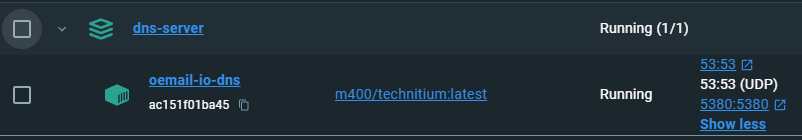
\includegraphics[width=0.9\textwidth]{docker-up-dns-server.png}
    \end{center}
\end{flushleft}

\section{Konfiguráció}
\begin{flushleft}
    Magát a konfigurációt webes környezetben hajthatjuk végre, amely látható is, hogy a \textbf{5380} porton fut. Cím, amelyen a konfigurációt elvégezhetjük:
    \begin{itemize}
        \item \verb|http://localhost:5380/|
    \end{itemize}
\end{flushleft}

\subsection{Zóna hozzáadása}
Megadott paraméterek:
\begin{itemize}
    \item Zóna neve: \verb|oemail.io|
    \item Típus: \verb|Primary Zone|
\end{itemize}

\subsection{Record hozzáadása}

\end{document}